\chapter{From ivory to silicone}
\label{chapter:conventional}

`Can you really feel the difference between the pianos?' Non-musician friends often found it strange that I queued up early in the morning to get one of my favorite rehearsal rooms at university. There are considerable differences between instruments. The keys, the sound, the smell, and how they are tuned all play a part in defining an instrument's `feel.' This is part of the tacit knowledge of musicians. Explorations into subjective experiences may help fill in some gaps missed by empirical research of other's experiences. In this chapter, I will describe my own experiences of playing with some commercial instruments and interfaces. While it feels daunting to use myself as an example, I have been inspired by others that have taken similar approaches.  \citet{sudnow_ways_1993,sudnow_ways_2001} describes learning jazz piano as an adult. \citet{aho_tangible_2016} tells the story of playing the Finnish kantele. Both of these are examples of approaching an instrument (and musical genre) as an adult. While they have been going into great detail about their journey of learning a particular instrument, I will provide a comparative perspective on playing multiple instruments.


\section{A techno-somatic approach}

Music evokes our senses and plays with our emotions. Philosophers have grappled with the question of emotions in music for millennia. Susanne \citet[p. 235]{langer_philosophy_1957} suggested that `music can \emph{reveal} the nature of feelings with a detail and truth that language cannot approach.' Many studies on affect and emotion in music focus on the music `itself.' Less attention has been devoted to the emotional experience of making music. As \citet{shaffer_cognition_1989} writes, music performance is not only about the mechanical production of notes. For a robot to play a Chopin waltz convincingly, it needs to have feelings about itself and the social context.

Music researchers generally do not spend much time thinking about instruments. Similarly, musical instrument researchers do not spend much time researching performance. I find this lack of interest in instruments and music performance strange. After all, instruments are essential to musicking. Also, if you ask musicians about their instruments, they could talk for days. They would most likely also become quite emotional during the conversation. Still, there is little research on emotions and affect related to instruments. What is it that makes us want to play specific instruments? Which features and qualities do these instruments have that others do not? Is it only the age and cost of an instrument that makes it desirable to play? Or the opposite, why are some instruments less engaging than others?

It should be no surprise that I believe the closeness between action and sound is part of one's \emph{affection} for an instrument. Of course, some of the basics of good instrument design should first be in place. \citet{sullivan_surveying_2019} found that professional musicians favor \emph{durability}, \emph{portability}, and \emph{ease of use} when choosing their instruments. These are all important factors, but I think it is critical also to consider what \citet{roads_computer_1996} describes as the `feel' in his classic Computer Music Tutorial:

\begin{quote}
Electronic input devices detach the control of sound from the need to power the sound; any one of dozens of input devices can control the same sound generator. This translates into musical flexibility. With electronic instruments, a single wind controller can create the low bass sounds as easily as the high soprano sounds. Creating extremely soft or loud sounds requires minimum effort since the control is electronic. Obviously, the detachment of sound control from sound production has a negative side---the reduction of the `feel’ associated with producing a certain kind of sound.
\end{quote}

These thoughts are equally valid today. The increased action--sound separation of new instruments has also decreased the feeling of \emph{inter}action when one plays an instrument. Playing the trumpet, one feels the lips' vibration towards the mouthpiece. It is a highly sensory experience and tightly coupled to the resulting sound. The same is usually not the case when playing an electro-acoustic instrument. But how does one explain such a `feel' of playing an instrument? In the following, I will present what can be called a \emph{techno-somatic} approach to borrow a term from \citet{paine_interaction_2015}. In my thinking, the meeting point between a user and the instrument can be broken down into three elements: the \emph{look}, the \emph{sound}, and the \emph{touch}. Together, these three elements constitute the `feel' of an instrument, as sketched in Figure~\ref{fig:feel}. We will, in the following, investigate these concepts in more detail.

 \begin{figure}[tp]
 	\centerline{
 		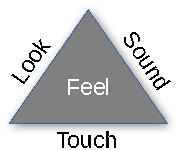
\includegraphics[width=.3\columnwidth]{figures/61-feel-crop.pdf}
 	\caption{The `feel' of an instrument can be understood as a combination of its `look,' `sound,' and `touch.'}
 	\label{fig:feel}
 	}
 \end{figure}


\subsection{The `look'}

Many people would probably argue that sound matters the most when `listening' to music. However, several studies have shown that vision matters more in music than we like to think. \citet{tsay_sight_2013} performed a series of experiments on conservatory competitions. In their self-reports, the expert judges said they focused most on sound in assessing the musicians. However, it turned out that visual information was the most important. Both novices and experts reliably identified the winners of the competitions from silent video recordings.

The visual importance of performance is reflected in the emphasis on stage setups, lighting, projections, extra video monitors, and so on in concert venues. Tickets are usually more expensive for positions where one can see the performers the best. For example, I prefer to sit on the center-left side of the hall when I go to piano concerts to maximize the possibility of seeing the finger action of the pianist. If going to a large stadium concert, I would instead position myself in the center to get a balanced view of both stage and monitors with close-ups of the performers.

The visual appearance of instruments also matter. The musical affordances are often conveyed through the instrument's physical construction. Thus, even before any sound has been made, the instrument's affordances have been `revealed' through sight. I think this matters to both performers and perceivers. Also, a designed object's color, shape, form, texture, and name tell something about who the object is made for and for what purpose. Most acoustic instruments have standardized shapes and colors, although there are some examples of violins painted red or pianos covered in silver. Such visual `hacking' is usually part of an artist's branding.

Electro-acoustic instruments are less standardized in their visual appearance, although many are based on keyboard designs or the `knobs-and-sliders' paradigm described in Chapter~\ref{chapter:mappings}. Many music technology devices also have a `techy' look. \citet{jawad_gatekeepers_2020} investigated how the color, form, and name of different music technologies affected peoples' gendered perception of the device. She selected nine example devices for an online gender assignment study and found that most were classified as male or neutral. Few were characterized as female. These findings correspond with general observations about the male-domination in the field of music technology  \citep{essl_gender_2003,born_music_2015,gadir_forty-seven_2017}.

Many traditional instruments are constructed so that it is possible to see the performance actions of the musician. That is not always the case with electro-acoustic instruments. For example, `knobs-and-sliders' controllers are usually not very audience-friendly. That may be one reason that several musicians have started to project close-up videos of their performance actions so that the audience can see what is going on. The same is the case in laptop performances. Live coders often project their screen for the audience to avoid being accused of `reading e-mail' on stage. That way, they can show how they are working with the sound-producing code. Other laptop performers have added visual elements to their performances, for example, projections of photos or abstract animations. There are several examples of outstanding audiovisual performances. However, I have been to performances with no apparent relationship between the visual and sonic elements. The visuals appear to have been added without much thought. Such audiovisual `dissonances' may ruin a performance. In some cases, it might be better to leave out the visuals. In fact, some performances of `tape music' are played in the dark. Then the audience is forced to focus on only listening.


\subsection{The `sound'}

The sound of an instrument is essential for how it feels, both to the performer and the perceiver. There are many levels of meaning to consider. One can think of the sound metaphorically (`a scary sound'), generally (`the sound of a synth'), related to the device (`an 808 sound'), or related to an artist (`the sound of Björk'). From a perceptual point of view, one can argue that the most important is the experienced sound (`the sound of a synthesizer connected to a medium-sized PA system in a small club with a semi-dry reverb').

Many instruments are claimed to have `unique' sound characteristics, and one of the strongest examples of this may be found within the world of violins. Here the old Italian violins, particularly the ones made by Stradivari, have an exceptional reputation. Just mentioning that someone plays a Stradivarius will make people sharpen their senses. The question is whether the fame of an instrument also primes the way the instrument is experienced. \citet{fritz_player_2012} called in for a double-blind test in which a group of 21 soloists evaluated six violins, three old ones (Stradivari and Guarneri del Gesu), and three new ones. They found that the new violins were repeatedly preferred above the old ones. The study received much attention and also criticism about the experimental setup. Therefore \citet{levitin_expert_2014} set up a new experiment to improve the experimental design on many of the criticized points. Now they had ten expert performers try six old and six new high-quality violins in two different venues. They came to the same conclusion; the new violins were systematically preferred over the old ones. In a third experiment, they followed up by checking the instruments' perceived quality by audience members \citep{fritz_listener_2017}. Again, the new violins were preferred to the old ones. While these findings caused harm, the researchers' main argument was not to devalue the old violins but to explain that new violins are equally good or better.
I think the findings from these violin studies are interesting because they show that knowledge of a brand may get in the way of the instruments' sonic qualities. Without the effect of the brand name, it boils down to the instruments' qualities.

Many electro-acoustic instruments have been built around specific sonic qualities. While only experts can discern the exact model names, many would probably recognize `the sound of the 80s' based on some synthesizer sounds. In some cases, companies may also brand their `sound' as different from others. For example, some might say that a Moog `sounds' different than a Roland synthesizer. That may be true, but there may be a share of corporate interests or ownership bias involved.


\subsection{The `touch'}

The third axis in my instrument `feel' triangle is \emph{touch}. The sense of touch is often broken down into three parts: \emph{cutaneous}, \emph{kinesthetic}, and \emph{haptic} \citep[p. 148]{weiner_handbook_2003}. The cutaneous system refers to the sensations in the skin, the tactile experience of the object one touches. The kinesthetic system refers to sensory input from the muscles, tendons, and joints. The haptic system combines the cutaneous and kinesthetic systems and is focused on actively touching and being touched. To generalize, we may say that the \emph{tactility} of an interface relates to what we feel with our skin, such as the surface material. The \emph{haptic} experience is related to how the surface moves, the vibrations we feel in our body, or the pressure exerted on our body from the interface itself.
Together, the combination of tactile and haptic experiences is part of what \citet{wang_artful_2018} calls the `resistance' of the interface.

The choice of material is essential for the overall tactile experience of an instrument. For example, think about the difference between touching wood, metal, or plastic. Even thinking about touching one of these surfaces will bring up mental images of how the materials feel. A metal object's flat and cold surface is undoubtedly different from the warm, textured wood feeling. The coating of the material also plays a role here. For example, the wood of an old scratched guitar is different from a shiny, new one. The size and form can also influence the way the instrument feels. The slides on my two trumpets are slightly different, making it necessary to adjust the hand position a little when I switch between them. These are tiny details, but they are still part of the `feel' of each instrument.

Although there are variations in tactile experiences between acoustic instruments, they are much more significant in electro-acoustic instruments. MIDI controllers come in all sizes, shapes, and materials: from the smallest, lightest controllers made of plastic to sturdy metal-based controllers with wooden elements. The latter would typically be the heaviest ones and would probably be perceived as more `expensive.' However, why? Because of the touch? Or weight?

Weight is a particularly tricky topic. In one way, one would assume that a heavy instrument is more sturdy. Some studies show how an object's weight leads to an increased feeling of monetary value \citep{jostmann_weight_2009}. On the other hand, we have been accustomed to smaller and lighter, yet more capable, devices through the digital revolution. A device's weight may also fool us. The plastic remote control for my new TV has a metal piece inside. The extra weight makes it sit better in hand. However, I would have preferred if the whole remote had been made of more sturdy materials. When it comes to instruments, heavier is not always better. If I can choose between two devices with different sizes and weights, I may be tempted to go for the lighter and smaller if it fulfills my needs. For musicians carrying their instruments around, size and weight are critical factors.

Up until now, we have primarily considered `static' touch properties of instruments. However, dynamic haptic feedback is also crucial for interaction. You get haptic feedback for `free' in acoustic instruments that the musician is holding or touching. However, as discussed in Chapter~\ref{sec:separation}, a larger action--sound separation will also lead to less haptic feedback. In electro-acoustic instruments, there may not be much haptic experience at all. Things are changing, though, and there has been a growing interest in haptic research over the last decades.
One of my favorite examples is the haptic FireFader by \citet{berdahl_firefader_2013}. This one-dimensional fader allows for creating powerful interactions based on providing haptic feedback with both a high spatial resolution and a high speed. % (Figure~\ref{fig:firefader}).
Combining this interface with a physical string model makes it possible to feel touching a `real' string. The Firefader provides only one-dimensional haptic feedback, but multi-point vibrotactile feedback solutions also exist. Musical haptics has up until now been a marginal research field but is quickly emerging \citep{papetti_musical_2018}. Successful research prototypes have shown that haptics is a viable path for the future of electro-acoustic instrument design. However, engineering difficulties and costs have hindered the development. The growing interest in haptics in other domains, particularly in the game industry, may help develop better actuator technologies and reduce the cost of integrating them into devices.


\section{From acoustic to hybrid pianos}

Keyboard-like musical instruments have a long and rich history \citep{keislar_history_1987}, and keyboard-based music controllers have been dominating electronic musical instrument designs for decades. Therefore it makes sense to start an analysis of commercial instruments from the perspective of the piano. I will use my former piano experience when going through different keyboard-based instruments, from my childhood acoustic piano to new electro-acoustic interfaces.


\subsection{Acoustic pianos}

In my childhood home, we had an old upright acoustic piano (Figure~\ref{fig:piano}). It had already lived a long life when I started playing on it and was completely worn out when I moved out of the house. I still have an embodied memory of sitting on the quirky chair and touching the keys on that piano. The ivory keys had a rich, physical texture. Many had scratches, and some even had cracks on the sides. Based on the recommendation of a piano tuner, the keys were replaced after some years. While the new, shiny, white plastic keys were an improvement in general, I remember that I missed the feel of the old ones. The tactile sensation of the old keys was terrific, although their unevenness became a problem when I started playing more rapidly.

\begin{figure}[tp]
 \centerline{
   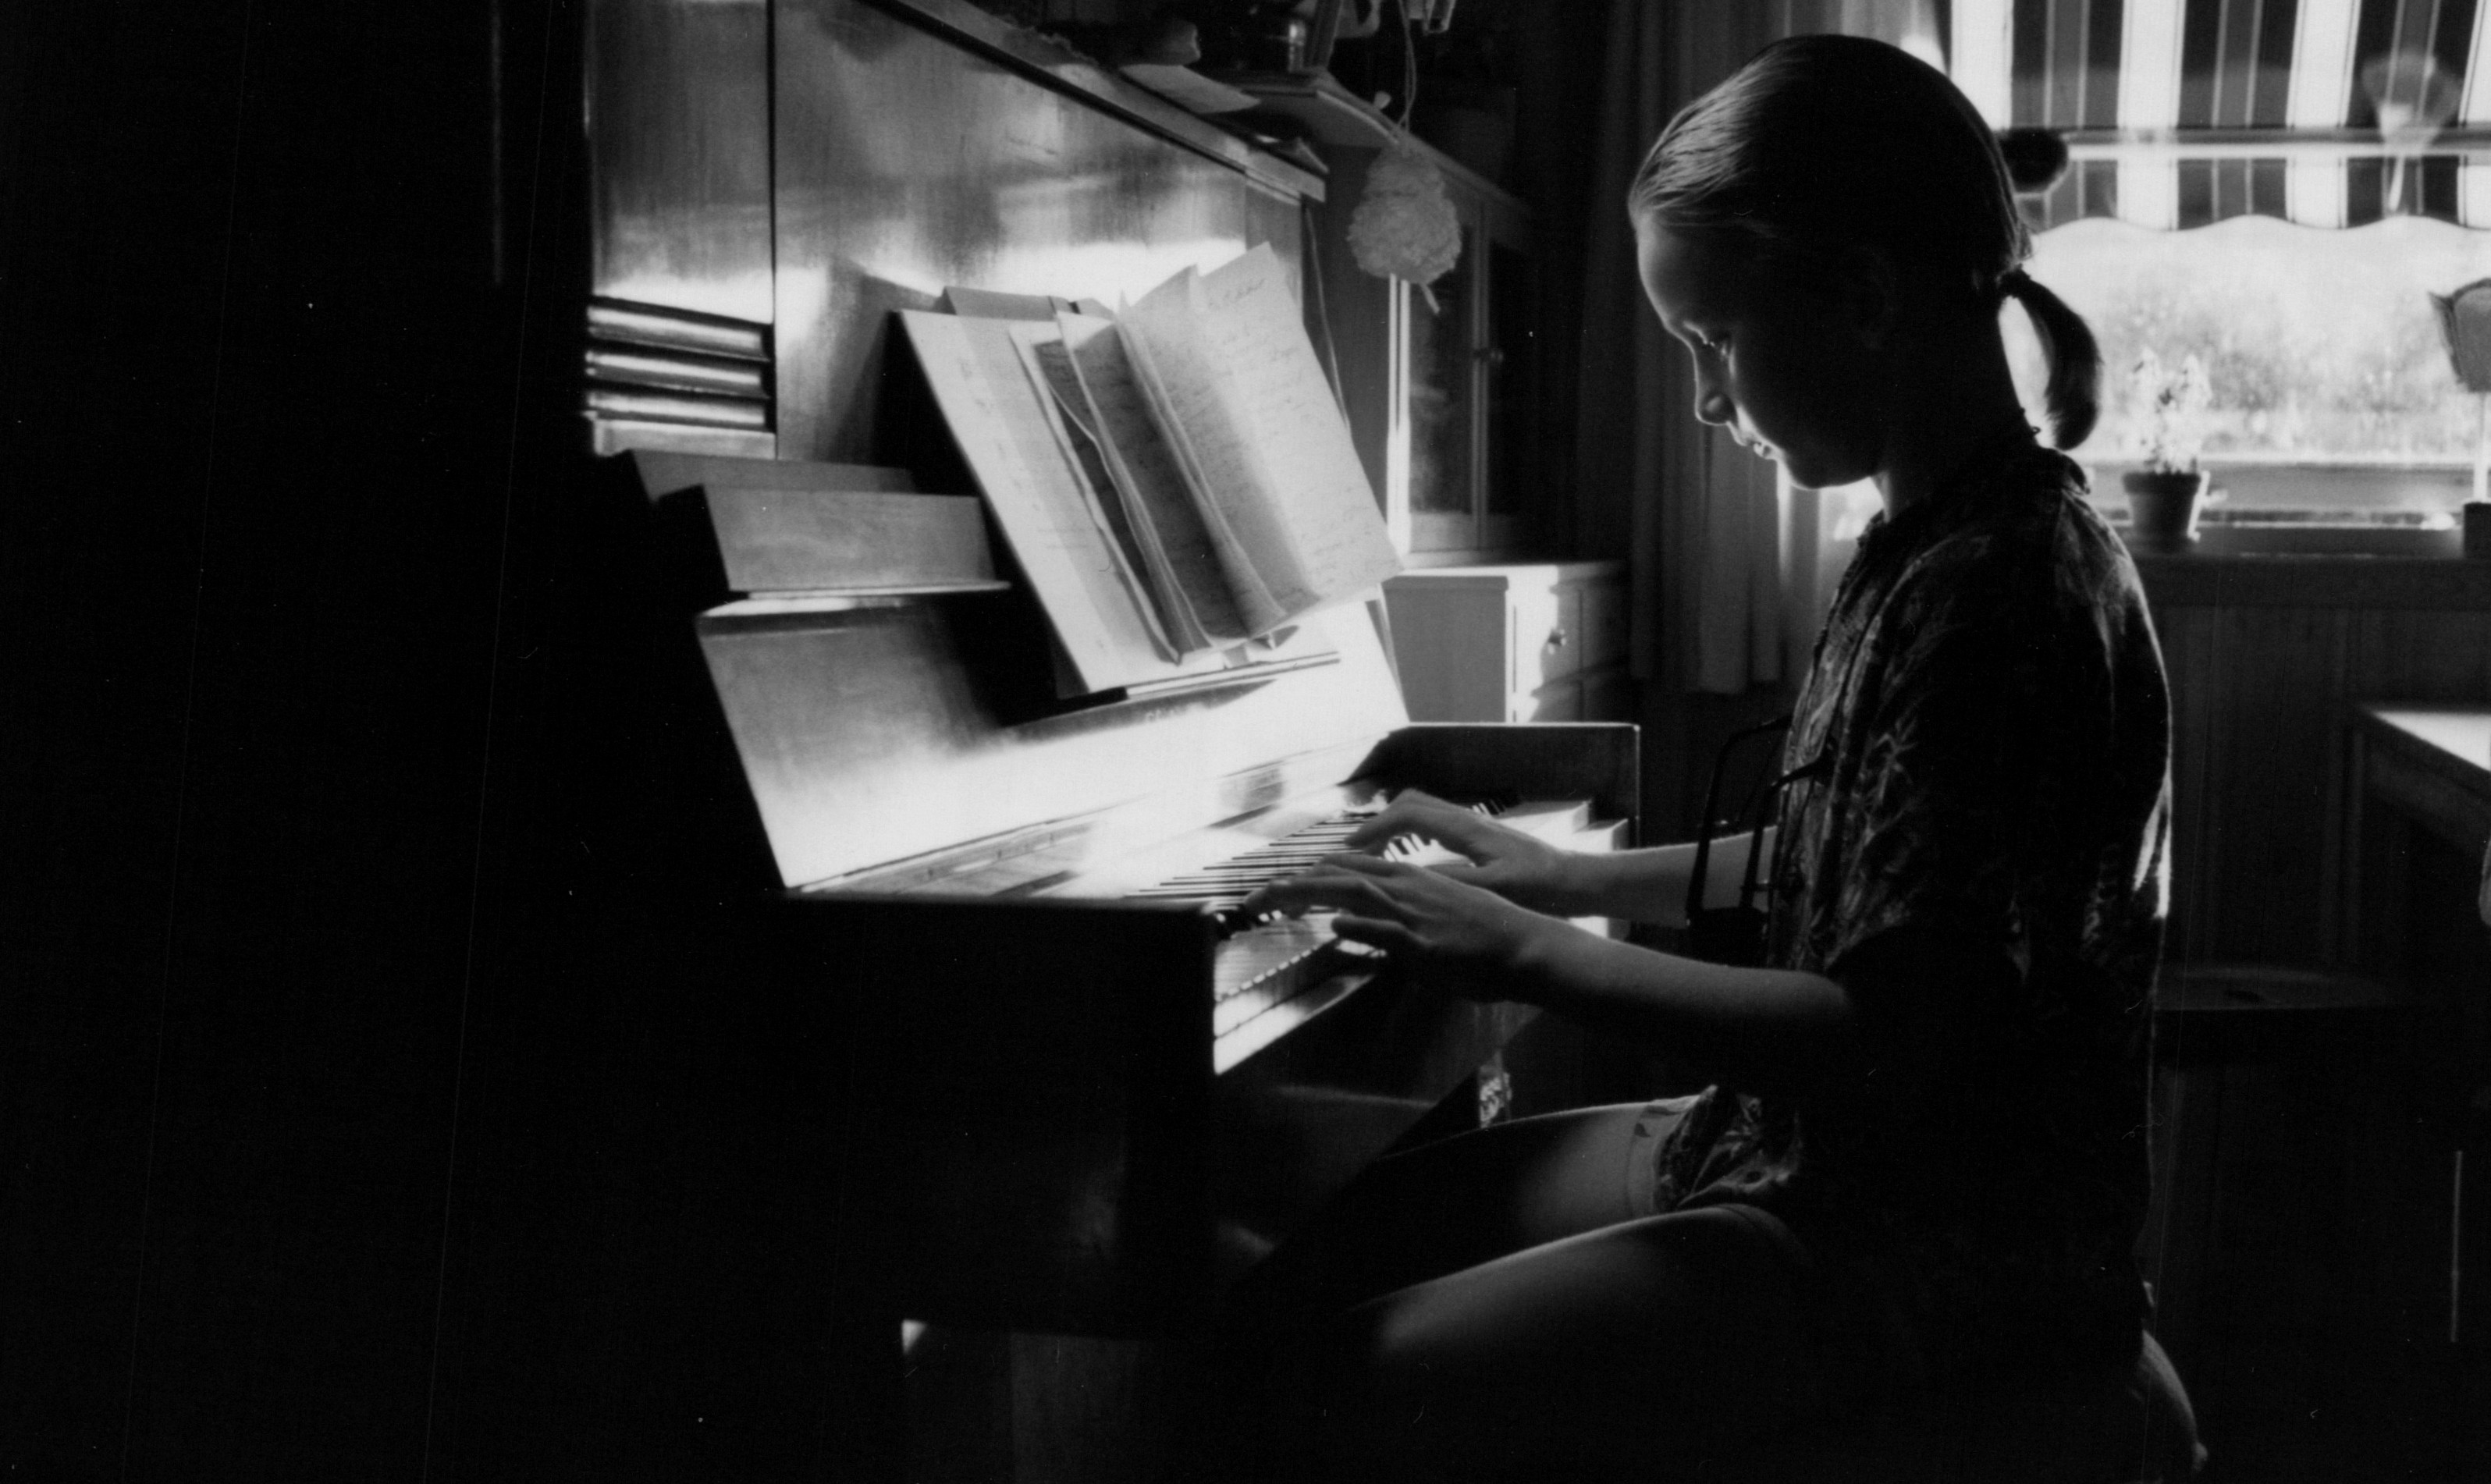
\includegraphics[width=\columnwidth]{figures/62-ivory.jpg}
 \caption{Practising on the old piano in my childhood home.}
 \label{fig:piano}
 }
\end{figure}

The felt on the hammers was also quite worn, and as I got older and started improvising more, I thought that the sound coming from the instrument was too dull. Sometimes when I was home alone, I removed the front plate to get more `punch' in the sound. This made the piano much loader, which was my primary motivation, but I also enjoyed watching the hammers move while playing. Already at that age, I was fascinated by the action--sound coupling of the hammer mechanism. Watching the hammers made me feel more connected with the instrument since I could see the sound-producing action.

The piano has a larger action--sound separation than what you find in embodied, tactile, and tool-based instruments. Still, the piano is a great first instrument. It has what \citet{wessel_problems_2002} call a `low entry fee.' Pressing a key will result in sound right away, and the logical layout makes it easy to start exploring melodic and harmonic relationships. A drawback of this `easy-to-get-started' factor is that pianists do not develop the same sensitivity to pitch---a keypress results in sound. You can modify the velocity of the keypress, which will alter the loudness of the tone, but you cannot change the tuning. If the tone is out of tune, you have to get used to it and wait until the next time the piano tuner comes around. When I started playing the guitar at the age of 12, I realized that I had been entirely ignorant of tuning. I had to work hard to incorporate a sensitivity to pitch. In contrast, those that play wind and string instruments spend a great deal of time learning to produce sound and intonate well.

On the positive side, playing the piano helps understand the basics of Western music theory: the relationship between notes, the distribution of notes in octaves, and chord structures. The drawback is that the piano effectively `locks' you into a Western music-theoretical paradigm and makes it difficult to experiment with non-diatonic tuning systems. My guitar teacher was a composer interested in alternative tuning systems, and he showed me how to tune the guitar differently and the effect this had on what I could play. I also learned to appreciate being in direct contact with the sound-producing elements with the guitar: touching the strings and feeling the guitar's vibrating body. Picking up the trumpet gave me an even closer physical sense of producing sound myself.

Instruments are different, and they influence the music you make with them. A benefit of playing the piano is that you become an `all-round' musician. Pianists often have good multitasking skills: creating a rhythmic pattern, balancing harmonies, and playing melodies. However, as I discovered when I started studying music, the drummers will always be better at rhythms, and the wind players will always be better at melodies. On the other hand, the pianists will team up with the guitarists in being good at harmony. The guitarists usually have a better ear, though, since they are used to tuning.

The instrument(s) you learn shape your musical expertise and experience.
Some people say that the instrument they play does not matter, that they have a musical idea in their mind and can play it on any instrument. For me, it is the opposite. The instrument I have at hand drives my musical creativity. Even when I try to play the same tune on another instrument, the result differs. The instruments have different qualities, and they afford other musical content and expression. To me, these possibilities and constraints of different instruments are attractive. The idiomaticity of various instruments gives them different musical affordances. That is why it is fun learning to play more instruments.

Many musicians are used to playing their own instruments, but pianists have to play on whatever instrument is available. The piano is one of a few instruments that musicians do not bring with them. There may be an economic benefit to not investing in a high-quality instrument on your own. The downside is that you rarely know what type of instrument you will play in a particular location. During my student days, I would chase for the rehearsal rooms with the best pianos. The pain of having to play on some of the worn-out or out-of-tune pianos was not tempting. The result was that I often played on 2--3 different pianos a day: my digital piano at home (more on that later), various upright pianos in the regular rehearsal rooms, and, when I was lucky, a grand piano in one of the large rehearsal rooms. Over the years, I have gained experiential knowledge of the qualities of various instruments. For example, playing an upright Yamaha piano with a `sharp' sound quality and heavy keyboard touch is undoubtedly different from playing a soft-touched Steinway grand piano. But even similar instruments from the same manufacturer differ. Acoustic pianos are unique instruments. Their differences may be minor, but they matter. Different touch and tone affect the musical result.

One of my favorite piano records---Keith Jarrett's Köln Concert---is an example of how a particular piano instrument greatly influenced the musical result. \citet{carr_keith_1992} writes about a misunderstanding about the instrument to be used for the performance. The instrument planned to use in performance was never moved to the Köln opera house. Instead, a small rehearsal piano was placed on the stage. This instrument was `thin' in the upper registers, weak in the bass, and had problems with the pedals. The mistake was discovered too late to make a replacement before the concert. Despite the difficulties, Keith Jarrett decided to play. The Köln Concert has become legendary. It stands out as quite different from his other solo improvisations, probably because he had to adjust his playing to the peculiarities of that particular piano.


\subsection{Digital keyboards}

After playing acoustic piano for some years, I got my first digital keyboard at around ten. It was a basic 3-octave keyboard with nine instrument banks and some basic drum patterns. It had a speaker built-in, so I would classify it as a complete electro-acoustic instrument. I still remember how strange it felt to touch the keys. At the time, I still played with the old ivory keys on the acoustic piano. The light keyboard keys felt slippery, and they gave no resistance compared to the acoustic piano. The disappointment with the keys quickly turned into the joy of exploring the keyboard's sonic possibilities. I particularly enjoyed playing with the different organ sounds. On the other hand, the `strings' never sounded like string instruments, and I was equally disappointed with the `wind' and `brass' sounds. However, the built-in drum machine was inspiring. The beats were basic, but they allowed for making up more complete songs. This was my first time exploring what I today would call a music-maker.

In high school, I became interested in exploring the possibilities of digital pianos, including making multitrack MIDI recordings. I saved up money from a summer job and bought a Roland RD-600 digital stage piano. I had read through all the reviews I could find in various music magazines and found it to be the best option given my budget. All the reviews had focused on the quality of the keys and the built-in sounds. What I had not thought about, which has resonated with me ever since, was that the piano did not have any built-in speakers. I guess it was evident to `everyone' that such a stage piano does not make any sound on its own. Connecting it to my Hi-Fi system worked, but playing over two relatively small speakers on the other side of the room was not a satisfactory experience. I ended up investing in a pair of good headphones to enjoy the high-quality sound. My regrets eventually ended, and I have had many good musical experiences with the RD-600 ever since. The keys were the best you could find on a digital piano at the time. They were undoubtedly a little more lightweight than on an acoustic piano, but this was easily compensated by the possibilities of changing between different sounds.

The RD-600 has been with me ever since. The lack of speakers still bothers me. I usually play it with headphones in my office, but it is more of a struggle to play something for others. Then I have to connect it to my small PA system to get sound. It is doable, but it keeps reminding me about the unnecessarily large action--sound separation. The counter-argument is that adding some small speakers into the RD-600 would be unnecessary, given that it was designed for stage usage. However, even on stage, some local speakers in the device could have been valuable. They could be used for warming up or to give some direct feedback to the performer. So the primary advice I give to everyone who wants to buy a digital piano is to get one with built-in speakers. That is, they should buy an \emph{instrument}, not only a controller or keyboard. Fortunately, many digital pianos sold these days have speakers built-in, although stage pianos and `synthesizers' typically ship without.


\subsection{Hybrid pianos}

I always dreamed about owning my own grand piano. For a long time, this was an unrealistic dream. Good grand pianos are expensive and require a lot of space. After moving to a new apartment some years ago, the dream could finally become a reality. The challenge, then, was to decide on an instrument. I ended up with a Yamaha N2 `hybrid piano.' This came as a big surprise to my surroundings, but also to myself. A few years earlier, I would never have thought to invest in a digital grand piano.
My three arguments for buying a digital piano were that it takes up less space than an acoustic grand piano, it does not need tuning, and the sound level can be adjusted. The latter is perhaps the most important when you live in an apartment. One of the reasons I have been able to play much over the last years is because I could turn down the volume not to disturb neighbors or wake up my daughters.

Before deciding what instrument to purchase, I spent time trying out all sorts of instruments in piano shops. Looking for acoustic instruments is challenging; they all have different characteristics. New instruments from the large manufacturers often have a `standardized' sound, but less `soul.' On the other hand, used grand pianos from smaller manufacturers may be too `soulful.' Parallel to trying acoustic grand pianos I also tested all the digital pianos I could find. None of the `normal' ones convinced me; the keys felt similar to the ones I already had on my RD-600. However, the `hybrid pianos' felt differently. These pianos have the complete hammer mechanism that you find in an acoustic grand piano. Other digital pianos often have some weight attached to the keys to make them feel piano-like. However, they still do not feel like acoustic pianos. Hybrid pianos are based on the same full-balanced keys that you would find in a regular grand piano. They also have small actuators sitting in the frame, making the keys vibrate while playing. This haptic feedback makes a tremendous difference when playing. It feels like playing on an acoustic instrument.

The second selling point (for me) of these hybrid instruments is the sizeable built-in speaker system. Most digital pianos are lightweight in comparison. This makes them easy to move around, but it also means that the instrument can move while playing. Stage pianos on a folding stand are the worst, as they typically wiggle back and forth while playing. Digital pianos with a built-in stand also feel more flimsy than an acoustic instrument. On the other hand, hybrid instruments have the same type of instrument body as acoustic pianos. That means that they have space for a good sound system, including good amplifiers and speakers. They also distribute the sound spatially. When playing on the right side of the piano, the sound comes from the right side of the instrument. So there is a spatial relationship between action and sound. A prominent bass speaker also helps get a real sense of depth in the instrument when playing in the bass register.

My N2 looks fine, but the sound and touch make it `feel' just right. It is not the same as an acoustic grand piano, but it is remarkably similar. I sometimes regret not having an acoustic grand piano. Having a perfectly tuned instrument is practical, but I miss the `soulfulness' of a slightly out-of-tune piano. For some time, I thought that the hammer action and sound were essential parts of why the instrument felt so natural. However, then the vibrotactile actuator system broke down, and I discovered how much the haptic feedback influences the instrument's feel. I also learned that such instruments need attention over time. Fortunately, parts can be replaced to get them back in order. So the touch is important for how such an instrument feels. However, the essential feature is the ability to turn down the sound level at night. It does not help the feel, but it makes me play.


\subsection{Electric pianos}

I have more experience with electro-acoustic pianos based on digital than analog circuitry. I have a couple of small analog synthesizers that I play with from time to time, but then I typically spend more time turning buttons than pressing keys. I think of them more as `synthesizers' than `pianos.' But I have one strong memory with an `electric piano.'

Some years ago, we rented a holiday apartment from a musician. In the corner of the apartment, partly hidden underneath a shelf and piles of books, stood a Wurlitzer electric piano. I had only briefly tested some old analog electro-acoustic pianos in the past. Now I had a chance to try one out for an entire week. The feel of playing on such an analog instrument is undoubtedly different from playing on a digital. People talk about the `character' of an instrument. To me, that boils down to its imperfections, whether in the look, the sound, or the touch. What made the Wurlitzer so enjoyable was that it was noisier than expected. It was slightly out of tune, and it had lots of scratches after being marked by many years' usage. It definitely looked and sounded more `authentic' than a digital piano.

I have fond memories of that week with the Wurlitzer, and it reminds me of the difference between analog and digital electronics. Analog electronics have some of those imperfections that you would also expect from acoustic instruments. That may be an asset in some cases but problematic in others. It is impossible to say that one instrument is better than another. All instruments have a different `feel,' and they all afford other types of musicking.


\section{Multidimensional controllers}\label{sec:mpe-instruments}

As described in Chapter~\ref{sect:midi}, MIDI Polyphonic Expression (MPE) has been developed to overcome some of the MIDI standard's limitations. New multidimensional controllers open for going beyond the impulsive sound-producing actions, predefined sound envelopes, and fixed amplitudes of traditional digital keyboard interfaces. These controllers are the result of several decades of research into alternative keyboard-designs, such as Multiply \citep{moog_multiply_1982}, a clavier optimized for curving pitch slides \citep{snell_sensors_1983}, Rolky \citep{johnstone_rolky_1985}, and Clavette \citep{fortuin_clavette_1995} to name a few. I call them `controllers' here since none contain speakers, and only a few contain a built-in sound engine. Over the last decades, we have seen several such multidimensional controllers reach the market, including
Continuum Fingerboard \citep{haken_indiscrete_1998},
Soundplane \citep{jones_force-sensitive_2009},
Seaboard \citep{lamb_seaboard_2011},
Touchkeys \citep{mcpherson_touchkeys_2012},
and Linnstrument \citep{linn_linnstrument_2013}.

Given my interest in keyboard-based instruments, I have followed the development of these new multidimensional controllers attentively. I will, in the following, reflect on my experiences with playing on several of these devices.


\subsection{A techno-cognitive approach}

My description of pianos earlier in this chapter focused on explaining the feel of the instruments using a techno-somatic approach. This was operationalized through the experiential parameters of look, sound, and touch. I could have used a similar method also when analyzing the multidimensional controllers. However, I decided to conduct the analysis using a techno-cognitive approach to understand their inner workings better. This was inspired by the work of a former master's student of mine, Mads Bye, who used \emph{dimension spaces} in an evaluation of multidimensional controllers \citep{bye_midi_2018}. He based his dimension spaces on the seven evaluation parameters proposed by \citet{birnbaum_towards_2005}. I will use a subset of these dimensions:

\begin{itemize}
	\item Plug-and-playability: the time and effort it takes to make the keyboard produce sound.

	\item Configurability: the number of modification possibilities used \emph{prior} to performing, such as setting up patches and loading samples.

	\item Controllability: the possibilities (and limitations) of the keyboard \emph{during} the performance, such as the number of keys and the multidimensional control of each key.

	\item Performability: the subjective experience of how the instrument works in a real-world musical setting.
\end{itemize}

The two first dimensions deal with what happens before performing. The plug-and-playability is essential when moving an instrument around. Sometimes time is not a limitation; other times, it is critical. Sometimes I have chosen to play with a different instrumental setup because I know there would be little time to set up before a performance. The plug-and-playability does not only relate to time. Complexity may also be an issue. Some keyboards may rely on a particular hardware and software combination to work. Then it may be easier to choose another more flexible one.

The configurability dimension also relates to setting up a device, but typically after it is already functioning. Selecting presets and loading samples may be seen as analogous to tuning an acoustic instrument. It typically happens before one plays or in between songs. With complex electro-acoustic setups, rehearsing what should happen between sets is critical. This could be seen as a type of non-real-time performance activity.

The controllability dimension may or may not overlap with the configurability dimension. The main difference is that the controllability dimension describes what happens \emph{during} a performance. In general, this may be the various types of continuous controls, such as pressing the keys on a keyboard instrument. But it may also include loading samples or loading presets on the fly.

Both the configurability and controllability dimensions can be thought of as describing the degrees of freedom of a device, albeit from different temporal perspectives (before and during a performance). In Chapter~\ref{sec:dof}, I defined the degrees of freedom as the number of independent movement variables in a mechanical system. This variable is relevant when considering the control dimensions of the device, which is a techno-cognitive term describing the possible usage of a device. Typically, more degrees of freedom of a system may correlate with a higher \emph{cognitive load} \citep{sweller_cognitive_1994}.

The number of degrees of freedom of a system is often challenging to operationalize. For example, how many degrees of freedom are there in a regular 88-note MIDI keyboard? There are 88 individual keys to choose between, so one may argue that it has 88 degrees of freedom. This makes sense if you think about the number of moving parts. However, each of the keys sends two control messages (pitch and velocity). Does this mean that you have 196 degrees of freedom? If we consider the usage of the controller instead of the device's construction, we may think about the hand's motion. Sideways motion controls the pitch selection, and vertical motion controls the velocity. Thus, one could argue that the controller only has 2 degrees of freedom (pitch and velocity). We should, in any case, also add the number of independent buttons and knobs on the device, such as data from the pitch wheel and connected pedals.

The exact number of degrees of freedom is less relevant than the complexity it reveals: the number of different `things' that the performer needs to consider while playing. Also, the complexity of an instrument does not equate with the complexity of the performed music. Good performers can create complex music with an instrument with few degrees of freedom. Similarly, a too complex instrument may not lead to any music at all if the performer cannot produce or control the sound. Thus, the optimal controllability of an instrument is often a sweet spot between its degrees of freedom and cognitive load.

\citet{fagereng_levende_2008} studied the performance setup of the Norwegian guitarist Eivind Aarset, a jazz musician known for working with many samplers and effects pedals. The study revealed that Aarset's arrangement increased in complexity over many years. Here complexity was defined as a combination of the number of devices, their degrees of freedom, and the cognitive load put on the performer. At some point, this complexity became counter-productive, and Aarset began scaling down the setup to (re)gain a level of control. In interviews, he confirmed that introducing constraints by removing gear and possibilities helped him be more creative in performance. So scoring high on configurability and controllability may, in many cases, lower an instrument's performability.

Many acoustic instruments can be thought of as having high plug-and-playability. For example, an acoustic guitar can be picked up and played (almost) right away. One may need to tune it, which could be seen as part of the configurability dimension. Still, a guitarist would be able to start playing within minutes of unpacking their instrument. The same is the case of a cellist, although a bit more preparation time is needed. First, you need to pick up the bow and tighten it by turning the tension screw. Next, you may need to apply rosin on the bow hairs. Then it is time to tune the strings.
Brass instruments can often be played quickly, and installing and wetting the reed of woodwinds does not take very long either. When they are ready, these acoustic instruments can be played for a whole concert without interruption. Some (re)tuning may be necessary between songs, but it is usually relatively quick. Brass players need to empty the spit valve, and others may need to adjust some mechanics. Occasionally, longer breaks are necessary, such as when a string breaks or a reed needs replacement. Still, the general level of performability is high in acoustic instruments.

The traditional instruments have been optimized and standardized for centuries. As such, they can be seen as having found different sweet spots between the various dimensions. In the world of electro-acoustic instruments, things are different. Many instruments have been designed and prototyped over the years, fewer have been produced commercially, but only some have become `mass products.' Thus, few electro-acoustic instruments---and here, I do not include hybrid instruments like the electric guitar---have been around long enough for performers to develop a career-long performance practice. A few professional musicians have specialized in playing early electro-acoustic instruments, such as the Theremin and Ondes Martenot. There are also some new interfaces for musical expression that have been used regularly, such as Michel Waisvisz' The Hands \citep{waisvisz_hands_1985}, Cléo Palacio-Quintin's Hyper-Flute \citep{palacio-quintin_eight_2008}, Hans Leeuw's Electrumpet \citep{leeuw_electrumpet_2012}, and Laetitia Sonami's Lady's Glove \citep{NIME20_45}. Except for the late Waisvisz, none of them have (yet) had time to develop a life-long relationship with these devices.

One could argue that keyboard players specialize in playing on electric pianos and synthesizers. However, most keyboard players change their setups over time. Many now also include computers as part of their instrument. This increases the configurability and controllability, albeit at the cost of plug-and-playability. For example, computer musicians may arguably be the most `flexible' in terms of what can be achieved on stage, but this often comes at the cost of long setup times. Driver problems are less problematic today than a decade ago, but I still frequently run into connection issues when setting up laptops with sound cards and controllers. Additionally, software needs to be started, sound files loaded, and mappings set up between controller and sound engine. Furthermore, even when everything is set up, there is always the risk of things not working. This is particularly the case when working with wireless and battery-powered devices. In comparison, bringing a hardware synthesizer to a gig is more comfortable. Then it may only be necessary to plug a power cable into a wall socket and connect a sound cable to the mixer. Some digital electro-acoustic instruments may be ready to play in seconds. Many mobile phone apps score high on plug-and-playability. A laptop can, too, if used without any peripherals. In most cases, a laptop will also be more configurable and controllable than a mobile phone. Whether that leads to a higher level of performability is another question. Sometimes they do, other times not. In my experience, playing laptop-based setups often rely on particular patches and ready-made material. Thus, the higher level of configurability leads to a longer time needed to move between settings in performance.

One often talks about the `expressive potential' of instruments. But what does that entail? \citet{dobrian_e_2006} questioned that many new digital controllers focus primarily on technical aspects. Less focus has been put into how we can make instruments that allow for expressive performance. Since then, there has been a growing body of research into using body control. This is an interesting line of work, and I will present some of my explorations into body-based instruments in Chapter~\ref{chap:touchless}. However, there is a misunderstanding that adding gestural control to an electro-acoustic will make it more expressive. That is built on the same misconception that adding more possibilities to a synthesizer will make it more performable. As \citet{magnusson_designing_2010} has argued, having endless possibilities may lead to a feeling of despair. He calls for the need to design constraints into new musical interfaces. Creativity blossoms if you work with a more limited instrument.

Interestingly, traditional acoustic instruments are full of constraints. In the mapping analyses by \citet{kvifte_instruments_1989}, most acoustic instruments have relatively few control dimensions. They also have a reasonably narrow action--sound palette. But why are such instruments then thought of as expressive? I would argue that expressivity is linked to a combination of an instrument's action--sound separation and the spatiotemporal distance between instrument and performer. You do not need a lot of options if the spatiotemporal resolution of the interaction is high. As such, all the multidimensional controllers in the following sections score higher than a traditional keyboard. They all allow for nuanced control possibilities, albeit in very different ways.


\subsection{McPherson's TouchKeys}

The first of the multidimensional controllers I will discuss in this chapter is TouchKeys by \citet{mcpherson_touchkeys_2012} (Figure~\ref{fig:touchkeys}). TouchKeys is different from the other included keyboards in that it is not a controller on its own. Instead, it is a regular MIDI keyboard controller with a set of key-shaped sensors glued on top of the keys. I have decided to include it here because it is a relevant `bridge' between a traditional digital keyboard and the MPE interfaces we will consider next.

\begin{figure}[tbp]
		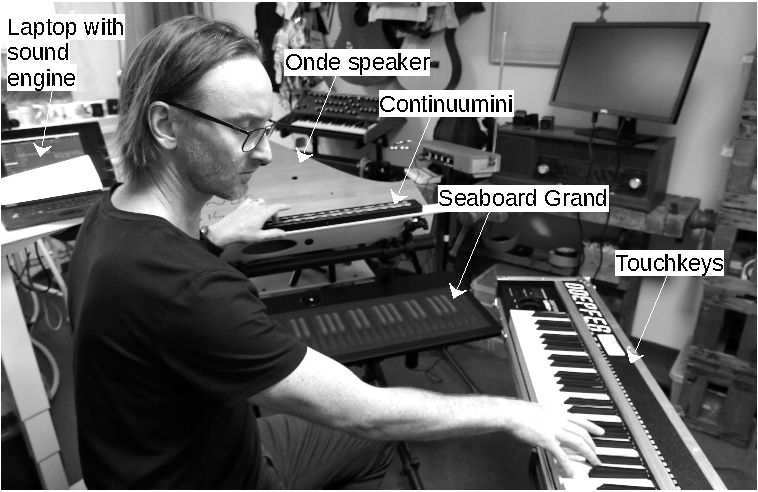
\includegraphics[width=1\columnwidth]{figures/63-mpe-instruments-crop.pdf}
	\caption{Playing with Touchkeys, Continuumini, and Roli Seaboard in the office. The devices are connected to an Onde loudspeaker.}
	\label{fig:touchkeys}
\end{figure}

The ToucKeys sensors allow tracking the XY position on each key. The input from the sensors comes in addition to the MIDI controller values from the keyboard itself. Therefore, ToucKeys behaves like a standard MIDI keyboard plus multidimensional control information for each key. The controller's plug-and-playability is relatively low since the values come in through two separate sources (MIDI input and sensor data input). It takes some time to use the data meaningfully. In fairness, TouchKeys should be seen as a research device more than a commercial product, so users would expect to know how to work with the data.

The controller itself does not allow for many configurations, and the controllability is limited to the user's programming. However, Touchkeys shines when it comes to performability. It can be played with a standard keyboard playing technique and allows for continuous sensing on each key.

The richness of the continuous sensor data streams is daunting at first. I always dreamed about continuously controlling the sound on each key on a keyboard. However, I never expected it to be so challenging to use in practice. At first, I started playing with a standard piano technique and tried to add various effects. The challenge is that playing with impulsive actions does not work well when you have continuous control. It is necessary to adopt a different playing technique to get something meaningful out of the controller.
I have found that the most interesting about TouchKeys is the ability to add vibrato and pitch shifts on individual keys.

% temporal adjustments
To avoid continuous control of each tone, I have found it necessary to program small `wait' commands before the continuous control kicks in. That means I can still play impulsive piano actions and get normal piano-like sounds if I play rapidly. However, when staying on a key, the continuous control will begin after a split second. This allows for a combination of impulsive and continuous control based on the temporal performance context.

% absolute vs. relative position
Pianists are used to dealing with discrete note values. You can press anywhere on the key and get the same tonal result. However, how does one handle the spatial (XY) sensor data? I have found it challenging to use absolute values when mapping continuous sensor data to sound parameters. Hitting a key in the same position without any reference point is impossible. For some sound parameters, such as a filter, it could work with using imprecise position control. However, for pitch shifting it makes more sense to calculate the relative distance from the initial pressure point. Still, it takes time to get used to thinking about both relative and absolute key positioning.

% number of fingers
When I first approached the TouchKeys, I used a standard piano technique with pressing anything from four to eight keys simultaneously. I quickly realized that having continuous control on each key results in a much higher cognitive load. Even after some time, I still have problems using much more than a few keys in a controlled manner. Playing sustained tones on a TouchKeys, you continuously need to consider the position and pressure level.

% sliding between keys
Another challenge is how to move between keys. It is possible to slide sideways on each key but impossible to slide between pressed and unpressed keys. This differentiates TouchKeys from some of the other `keyless' multidimensional controllers. TouchKeys biggest strength may be that it allows for using a traditional keyboard technique. This may also be its main limitation since it effectively hinders utilizing the full potential of its sensing capabilities.

% touch
The touch of TouchKeys is quite different from what I am used to from pianos and keyboards. The TouchKeys sensors are made of plastic but have another coating than regular keyboards. Each key is also perforated, making them feel more sticky than other keyboard controllers.

% conclusion
The TouchKeys was the first multidimensional controller I played, and it opened my eyes to the world of continuous keyboard control. I have had a great time exploring its possibilities and limitations. At first, I naively thought adding continuous control to all keys would make such a piano-like controller more expressive. I have had to adjust my expectations and understand why all the new MPE controllers have opted for designs that deviate from a traditional keyboard design.


\subsection{Roli's Seaboard Grand}\label{sec:seaboard}

My first encounter with the Roli Seaboard was during the International Conference on New Interfaces for Musical Expression in Oslo in 2011. \citet{lamb_seaboard_2011} presented a prototype of a silicone-based piano claviature and later commercialized the product. There are nowadays several different versions of the controller. I purchased one of the early ROLI Seaboard Grand devices, a 61-note controller that has later been discontinued (Figure~\ref{fig:touchkeys}).
The Seaboard does not have individual keys. Instead, it is built around a continuous silicon surface with `bumps' indicating the keys. The softness of the surface makes for a different tactile experience. One almost gets the sense of `faux' haptic feedback when pressing hard into the surface. One compelling design feature is that the silicone material and sensing extend beyond the multidimensional keys. This allows for using the upper and lower part of the keyboard as long touch strips.

When it comes to plug-and-playability, the Seaboard Grand scores high. It does not have a built-in speaker, so you still need to connect it to headphones or an external speaker system. However, with a built-in synthesizer, you can start making sounds right away. New versions of the Seaboard do not have a built-in sound engine, which means that you rely on an external sound engine to produce sound. To me, this makes a difference. I connect the Seaboard to a laptop once in a while, but I play with its internal sound engine much more times. That is why the Seaboard is one of the alternate controllers I have played the most, and it is the one I typically showcase when I have visitors in my office.

The levels of controllability and configurability on the device itself are not exceptionally high. There is volume control, and it is possible to change between sound presets. Many varied presets make it possible to produce many different sounds, most of which utilize the multidimensional control possibilities. Of course, connecting to software makes it possible to fully explore the potential of both the controller and the sound engine. I find it is interesting that the sound engine has been developed specifically to explore the multidimensional control possibilities. The Seaboard was developed before the MPE standard, and there were few multidimensional sound engines around. So it was necessary to think about both action and sound to realize the potential of this novel controller.

When I received the Seaboard, I thought the piano-like keyboard would make it easy to play. However, playing scales on the soft keys requires practice. This is even more evident when playing chords. Finger placement is easy, but intonation is difficult. At first, I thought that the possibility to slide between individual keys was exciting, but I have found it is easier to play with sliding-like actions above or below the keys. That extended area functions as a long touch strip. Then it is possible to get the sense of playing a sustained instrument rather than just pressing on/off on a controller.
As for performability, one thing that helps when playing tonal music is the `pitch lock-in' feature on individual notes. This feature makes it easy to play in tune, but it is also a limitation if one wants to play more freely. There is a similar type of lock-in feature when sliding an octave. It is, of course, possible to program it otherwise (in software), but I have come to see these features as idiomatic to the device.

All in all, the Seaboard is fun to play. Being able to have multidimensional sound control is immediately rewarding. The lock-in features make it easy to get started and results in few surprising results or false triggering. Even though it is easy to get started, it is not an easy instrument to master. I have found that having a piano background only partially helps. Multidimensional control is quite different in practice. As for the feel, the Seaboard is unique. The metal casing is sturdy and feels solid, and the touch of the silicone surface is quite unlike anything else I have played. It also looks different, which adds to the package.


\subsection{Madrona Labs' Soundplane}

The Soundplane was described as a `force-sensitive surface for intimate control' when it was first presented by \citet{jones_force-sensitive_2009}. It has later been commercialized by Madrona Labs (Figure~\ref{fig:soundplane}). The controller has 150 `pads' that respond to velocity, pressure, and two-dimensional position tracking. What makes this controller unique is the playing surface, which is made entirely out of walnut wood. This gives it a look, touch, and smell that resembles acoustic instruments.

The plug-and-playability is relatively low. The Soundplane has no inputs or outputs except for a USB port for communication and bus power. It relies on proprietary OSX software, which only handles the parsing of control data. So you need an additional sound engine to make it work. There are no onboard controls for alternative configuration modes, and the software editor also has limited alterations, so it also scores low on configurability and controllability.

\begin{figure}[tbp]
		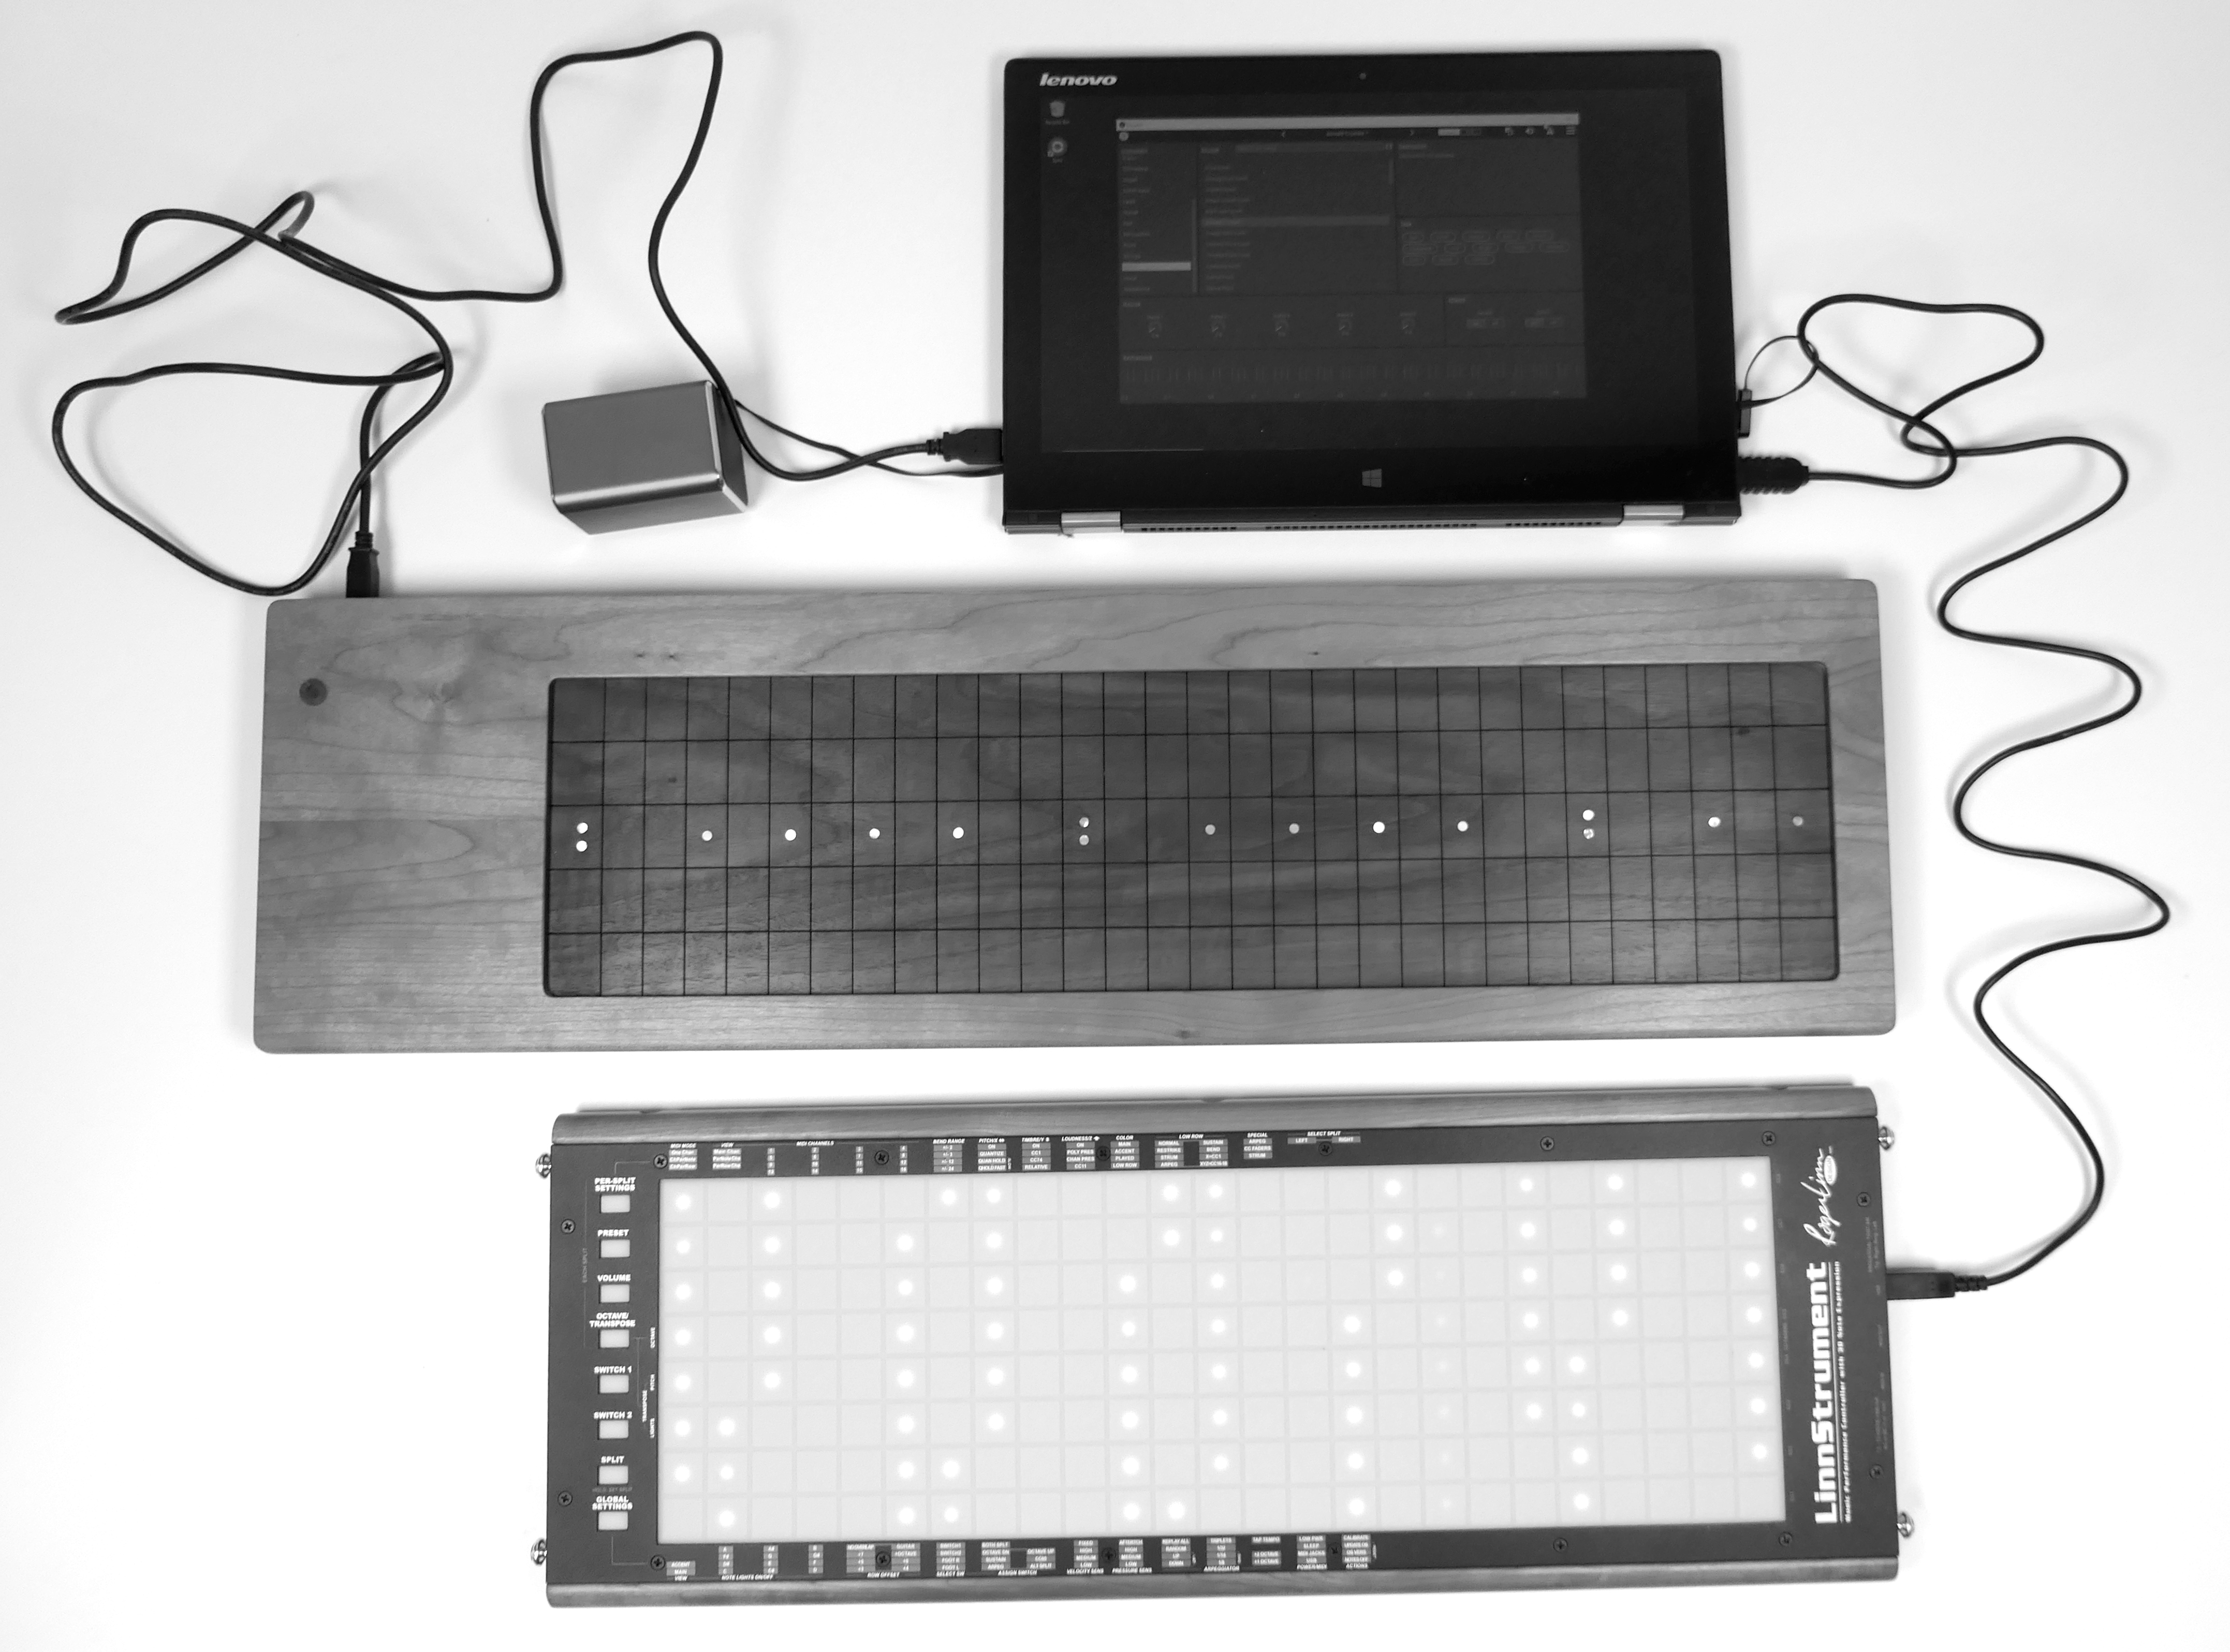
\includegraphics[width=1\columnwidth]{figures/64-linnstrument-soundplane.jpg}
	\caption{The Linnstrument (bottom) and Soundplane (middle) are examples of multidimensional grid-based controllers. They rely on a computer running a sound engine and a speaker to make sound.}
	\label{fig:soundplane}
\end{figure}


Fortunately, the Soundplane shines when it comes to performability. In many ways, it is the opposite of the Seaboard. The flat control surface of the Soundplane invites continuous control beyond the `keys.' There are small gaps between the keypads, but it is easy to slide between them. It is tricky to play individual notes, scales, and chords; the Soundplane works much better for timbral and textural control. Like with the TouchKeys and Seaboard, I find it challenging to handle more than a couple of continuous tones simultaneously.

What works well with the Soundplane is the controller's high spatial and temporal resolution and low latency. This makes it possible to explore sonic features with a high level of detail. The Soundplane is my controller of choice if I want to test a sophisticated sound engine. I often tell my students that even the most basic sound engine can come `alive' with a high-quality controller. The high spatiotemporal resolution of the Soundplane affords inspiring sonic results.


\subsection{Roger Linn's Linnstrument}

The Linnstrument 128 is an MPE-compatible controller with 128 RGB back-lit rubber pads (Figure~\ref{fig:soundplane}). The pads respond to velocity, pressure, two-dimensional position, and release velocity. The controller connects to the computer via USB and is bus-powered. As such, it resembles the Soundplane in many ways. It is about the same size and also has a grid-like construction. However, there are many differences.

The fact that the Linnstrument can function as a regular MIDI device right away makes the plug-and-playability of the controller much higher than the previously mentioned controllers. You still need to connect it to both a sound engine and speakers, but that is easier with generic MIDI support. Enabling the MPE mode requires extra fiddling, so I would give it an average `score' on the plug-and-playability dimension.

While the Soundplane relies entirely on software for configuration and control, Linnstrument has many more options built into the controller itself. It is possible to change the tuning of the pads, split the layout, use the built-in arpeggiator, step sequencer, `strum'  mode, and so on from the controller itself. It takes time to understand how these settings work. However, once learned, you can change a lot of settings on the controller.

At first, I thought that the RGB-lit plastic pads were a bit `cheesy.' For example, the Soundplane's wood surface feels so much more organic in comparison. However, I have found that the slightly elevated keys make playing tones, scales, and chords much more straightforward. The fact that keys light up in octave relationships makes it easy to jump around on the surface. Playing chords is more challenging. Unlike the highly sensitive Soundplane, the pads on the Linnstrument require a certain level of touch to be activated. The keypads feel a little stiff, but the response is consistent. Since there is a clear gap between keypads, the controller feels more key-based than continuous. It is possible to slide between keys, but it does not feel natural. That said, the Linnstrument scores high on performability. It is easy to navigate even after a short practice time, and it feels musical right from the start.


\subsection{Haken Audio's Continuumini}

The Continuumini is a controller produced by Haken Audio (Figure~\ref{fig:touchkeys}). It is the `little sister' of the piano-sized Continuum Fingerboard but otherwise shares many of the same properties. It is made of metal and has a flat felt-like playing surface. It is perceived as a sturdy device with a tactile feel.

Like the Seaboard Grand, the Continuumini has a built-in synthesizer. There are no speakers, but the addition of a sound engine makes it possible to play without a computer. This also leads to a `zero-latency' feel when playing.
The Continuumini has few options for configuration beyond changing presets. It allows for changing octaves on the device, which is practical for such a small control surface, but otherwise relies on configuration options in the software editor.

As opposed to the other controllers discussed here, the playing surface on the Continuumini is so tiny that it primarily affords to play with one or two fingers at a time. At first, I thought that this would be a limitation. However, given the high spatiotemporal resolution of the device, more focus goes into shaping individual tones through continuous control.

Continuumini's control surface is connected to mechanical springs, so the whole surface moves up and down when playing. This results in some mechanical `noise,' which I find charming given the controller's otherwise digital nature. The springs also give some resistance, so even though there is no digital haptic feedback, the controller has mechanical feedback.

When it comes to performability, the Continuumini is a rewarding controller. I am still working through the myriads of presets on the device and have found many smart mappings. For example, several of the presets allow for playing both with impulsive and sustained actions. This is a similar type of mapping that I ended up making for the TouchKeys. The result is that it is possible to play impulsive-like sounds with impulsive actions while at the same time being able to stop in one position and work with sustained control. The addition of various after-touch features that start when one lifts a finger from the surface is also cleverly programmed. All in all, the device feels very musical.


\subsection{Comparing apples and pears}

The above-mentioned multidimensional controllers are the first of a new generation of commercial music technology devices. The advent of the MPE standard means that many more will probably be produced in the coming years. While the existing devices share some characteristics, there are also many differences. That is refreshing, given that MIDI controllers have become fairly standardized over the years. I will not dwell too much on discussing details that will quickly be obsolete. I am more interested in reflecting on some of the techno-somatic properties of such multidimensional controllers.

Let us start by considering the \emph{look} of the devices. While plastic has taken over as the primary construction material in many commercial products in the last decades, I have been positively surprised to see products manufactured in metal and wood. However, using such materials is costly. It should be noted that these controllers are exclusive products and are not priced to meet the mass market. Still, I hope that we can get to a point at which solid construction becomes viable again. After all, considering the time it takes to master a musical instrument, they should be built to last. This is also important from a climate perspective. It is not sustainable to continuously make new products that break after a short period of usage. In addition to the more robust construction, working towards standardization of communication protocols and software-based updates may also help keep controllers alive longer than they have been over the past decades.

The materials used in a controller also influence their \emph{touch}. Again, I have been positively surprised by the variety of materials used in the playing surfaces in these multidimensional controllers: rubber, silicone, wood, and felt. This leads to a different playing experience than you usually get with plastic-based controllers. It certainly feels liberating and gives each of the controllers its unique tactile signature. Some of them even have a sense of haptic feedback, such as Soundplane's silicone-based keys and Continuumini's spring-based surface. The Linnstrument does not have such haptic feedback, but the light feedback on each key works well. Since the playing surface is otherwise just a grid of white buttons, it helps that the buttons light up to show adjacent tones and octaves.

Since none of the controllers have built-in speakers, and only two of them have built-in sound engines, it is impossible to compare their \emph{sound}. It should be clear by now that I favor instruments that produce sound on their own. Seaboard and Continuumini have built-in synthesizers that are optimized for their control capabilities. I can use these controllers also with generic sound engines, but I enjoy exploring the mappings developed by the instrument makers. This gives these particular controllers more of a musical identity. There is also a practical component to this. The plug-and-playability is much higher when you just need to turn on a device to make sound. There is no need to turn on a laptop, connect the device and start up one or more software packages to make everything work. Having a built-in sound engine also helps to lower the latency in the system. Even though they do not have built-in speakers, they feel more like complete instruments. In practice, I see that I play the Seaboard and Continuumini more than the other controllers.

Given that all the devices allow for controlling multidimensional sound engines, it has been fascinating to explore the same sound engines with each device. This has made me realize how much a controller influences sound production. You would imagine that playing the same sound engine with similar controllers would result in the same sonic and musical results. However, as I have spent time getting to know each of the controllers, I have realized that they afford different types of sonic control. For example, the Soundplane lends itself better to continuous control of timbres and textures, while the Linnstrument is the one to reach for when playing traditional melodies and harmonies.

Another general impression is that the multidimensional controllers provide excellent control over pitch and timbre. Paradoxically, this continuous control also limits the number of tones that can be played simultaneously. Before I started playing such devices, I thought multidimensional control would allow me to play like a pianist with timbral superpowers. Instead, I have found myself hitting the techno-cognitive `glass ceiling.' \citet{miller_magical_1956} elegantly summarized the limits of human information processing capacity as `the magical number seven, plus or minus two.' On a regular piano, I can easily play harmonic progressions with seven tones at a time. However, on these multidimensional controllers, I typically play one or a few tones at a time. I have found it impossible to play full chords with individual intonation on each tone. This is something that musicians playing on continuous-control acoustic instruments could have quickly informed me. After all, they spend an entire life playing one---or only a few---tones at a time.
